 \documentclass{article}
\usepackage[utf8]{inputenc}
\usepackage[a4paper, total={7in, 10in}]{geometry}
\usepackage{braket}
\usepackage{xcolor}
\usepackage{amsmath}
\usepackage{amssymb}
\usepackage{amsfonts}
\usepackage{graphicx}
\usepackage{svg}
\usepackage{float}
\usepackage{tikz}
\usepackage[ruled,vlined]{algorithm2e}
\usepackage{multicol}
\usepackage[backend=biber,style=alphabetic,sorting=ynt]{biblatex}
\usepackage{xcolor}
%\addbibresource{sample.bib} %Import the bibliography file

\newcommand{\commentt}[1]{\textcolor{blue}{ \textbf{[COMMENT]} #1}}
\newcommand{\ctt}[1]{\commentt{#1}}
\newcommand{\prb}[1]{ \mathbf{Pr} \left[ {#1} \right]}
\newcommand{\onotation}[1]{\(\mathcal{O} \left( {#1}  \right) \)}
\newcommand{\ona}[1]{\onotation{#1}}
\newcommand{\PSI}{{\ket{\psi}}}
\newcommand{\LESn}{\ket{\psi_n}}
\newcommand{\LESa}{\ket{\phi_n}}
\newcommand{\LESs}{\frac{1}{\sqrt{n}}\sum_{i}{\ket{\left(0^{i}10^{n-i}\right)^{n}}}}
\newcommand{\Hn}{\mathcal{H}_{n}}
\newcommand{\Ep}{\frac{1}{\sqrt{2^n}}\sum^{2^n}_{x}{ \ket{xx}}}
\newcommand{\HON}{\ket{\psi_{\text{honest}}}}
\newcommand{\Lemma}{\paragraph{Lemma.}}


\setlength{\columnsep}{0.6cm}

\newcommand{\Gz}{ G_{z}^{\delta} } 

\begin{document}

\title{Quantum LTC With Positive Rate}
\author{David Ponarovsky}
\maketitle
\begin{multicols*}{2}
\newcommand{ \Hw }{ \delta\Delta -\Delta^{\frac{1}{2}-\varepsilon}/\delta  }
	\newcommand{ \Nw }{ \Delta^{\frac{3}{2}-\varepsilon}} 
	  \newcommand{ \Gu } { \Gamma^{\cup} }
	  \newcommand{ \Guq } { \Gamma^{\cup, \square} }

    	\newcommand{ \Gsa } {\Gamma_{\square_{1}} }
	\newcommand{ \Gsb } {\Gamma_{\square_{2}} }
        \newcommand{ \Aa } { C_{A_{1}}}  
	\newcommand{ \Ab } { C_{A_{2}}}
	\newcommand{ \Ac } { C_{A_{3}}}
	\newcommand{ \Aab } { \Aa \otimes \Ab } 
	\newcommand{ \Aac } { \Aa \otimes \Ac }
	\newcommand{ \Aabc } { \Aa \otimes \Ab \otimes \Ac }
	\newcommand{ \Aabp } { \Aa^{\perp} \otimes \Ab^{\perp} } 
	\newcommand{ \Aacp } { \Aa^{\perp} \otimes \Ac^{\perp} }
	\newcommand{ \Aabcp } { \Aa^{\perp} \otimes \Ab^{\perp} \otimes \Ac^{\perp} }
	\newcommand{ \Aabpp } { \left( \Aabp \right)^\perp } 
	\newcommand{ \Aacpp } { \left( \Aacp \right)^\perp }
	\newcommand{ \Aabcpp } { \left( \Aabcp \right)^\perp }
	\newcommand{ \YY } {  y_{1}y_{2}^{\top} }
	\newcommand{ \ZZ } {  z_{1}z_{2}^{\top} } 
	\newcommand{ \TT } { \tilde{\tau} } 


  \paragraph{preamble.} preamble.  
  \begin{figure}[H]
            %\label{fig:square}
            \begin{center}
            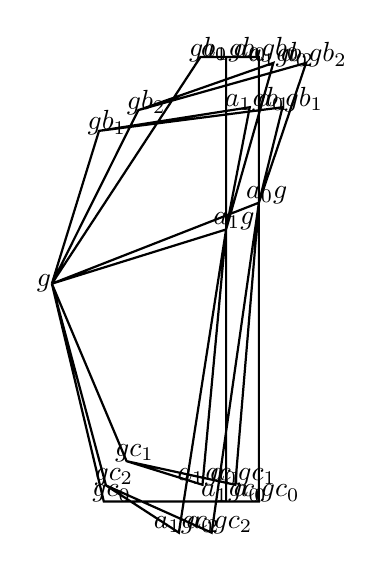
\begin{tikzpicture}
            \draw[thick](0,0)(0,0) -- (1.8868909852799058,2.877865480895461) -- (2.6291020107727636,2.877865480895461) -- (2.6291020107727636,1.0284276318890135) -- (0,0)
(0,0) -- (0.5987042288411264,1.940529734273733) -- (2.9291020107727634,2.240529734273733) -- (2.6291020107727636,1.0284276318890135) -- (0,0)
(0,0) -- (1.098226261405628,2.2039159134751554) -- (3.2291020107727637,2.8039159134751555) -- (2.6291020107727636,1.0284276318890135) -- (0,0)
(0,0) -- (1.8868909852799058,2.877865480895461) -- (2.212829904199719,2.877865480895461) -- (2.212829904199719,0.688600415063617) -- (0,0)
(0,0) -- (0.5987042288411264,1.940529734273733) -- (2.5128299041997186,2.240529734273733) -- (2.212829904199719,0.688600415063617) -- (0,0)
(0,0) -- (1.098226261405628,2.2039159134751554) -- (2.812829904199719,2.8039159134751555) -- (2.212829904199719,0.688600415063617) -- (0,0)
(0,0) -- (0.6596595875403375,-2.7665248409603684) -- (2.6291020107727636,-2.7665248409603684) -- (2.6291020107727636,1.0284276318890135) -- (0,0)
(0,0) -- (0.9489317965989157,-2.253957853716349) -- (2.329102010772764,-2.5539578537163488) -- (2.6291020107727636,1.0284276318890135) -- (0,0)
(0,0) -- (0.687195544150421,-2.5620796445105336) -- (2.0291020107727635,-3.1620796445105337) -- (2.6291020107727636,1.0284276318890135) -- (0,0)
(0,0) -- (0.6596595875403375,-2.7665248409603684) -- (2.212829904199719,-2.7665248409603684) -- (2.212829904199719,0.688600415063617) -- (0,0)
(0,0) -- (0.9489317965989157,-2.253957853716349) -- (1.9128299041997188,-2.5539578537163488) -- (2.212829904199719,0.688600415063617) -- (0,0)
(0,0) -- (0.687195544150421,-2.5620796445105336) -- (1.6128299041997187,-3.1620796445105337) -- (2.212829904199719,0.688600415063617) -- (0,0)
;
\node at (2.7291020107727637,2.977865480895461) {$ a_{ 0  } gb_{ 0 } $};
\node at (3.0291020107727635,2.340529734273733) {$ a_{ 0  } gb_{ 1 } $};
\node at (3.329102010772764,2.9039159134751555) {$ a_{ 0  } gb_{ 2 } $};
\node at (2.312829904199719,2.977865480895461) {$ a_{ 1  } gb_{ 0 } $};
\node at (2.6128299041997187,2.340529734273733) {$ a_{ 1  } gb_{ 1 } $};
\node at (2.912829904199719,2.9039159134751555) {$ a_{ 1  } gb_{ 2 } $};
\node at (2.7291020107727637,-2.6665248409603683) {$ a_{ 0  } gc_{ 0 } $};
\node at (2.429102010772764,-2.4539578537163487) {$ a_{ 0  } gc_{ 1 } $};
\node at (2.1291020107727636,-3.0620796445105336) {$ a_{ 0  } gc_{ 2 } $};
\node at (2.312829904199719,-2.6665248409603683) {$ a_{ 1  } gc_{ 0 } $};
\node at (2.0128299041997186,-2.4539578537163487) {$ a_{ 1  } gc_{ 1 } $};
\node at (1.7128299041997188,-3.0620796445105336) {$ a_{ 1  } gc_{ 2 } $};
\node at (-0.1,0) {$ g $};
\node at (2.7291020107727637,1.1284276318890136) {$ a_{ 0 }g $};
\node at (2.312829904199719,0.788600415063617) {$ a_{ 1 }g $};
\node at (1.986890985279906,2.977865480895461) {$ gb_{ 0 } $};
\node at (0.6987042288411264,2.040529734273733) {$ gb_{ 1 } $};
\node at (1.198226261405628,2.3039159134751555) {$ gb_{ 2 } $};
\node at (0.7596595875403375,-2.6665248409603683) {$ gc_{ 0 } $};
\node at (1.0489317965989158,-2.153957853716349) {$ gc_{ 1 } $};
\node at (0.7871955441504209,-2.4620796445105335) {$ gc_{ 2 } $};

            \end{tikzpicture}
            \end{center}
            \caption{Square of the complex, with edges $(g,ag), (agb, gb) \in E_A,
            (g,gb), (agb, ag) \in E_B.$ \label{fig:square}
            }
            \end{figure}
 \begin{figure}[H]
            %\label{fig:square}
            \begin{center}
            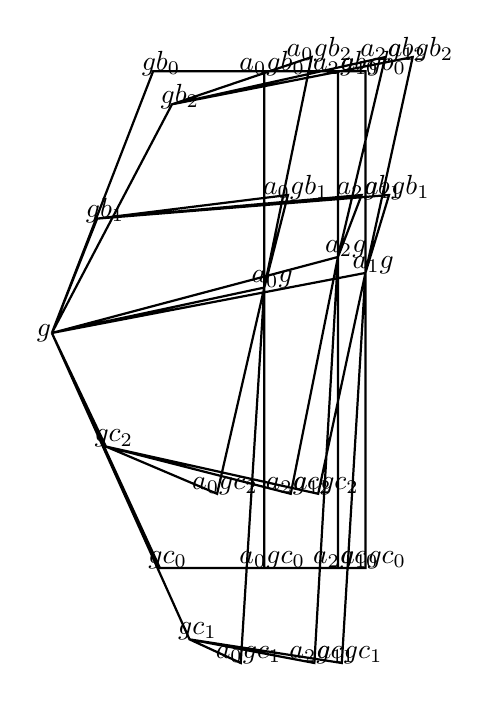
\begin{tikzpicture}
            \draw[thick](0,0)(0,0) -- (1.2862782871640814,3.3250342667862864) -- (2.6982935114146365,3.3250342667862864) -- (2.6982935114146365,0.5770015155690579) -- (0,0)
(0,0) -- (0.5754360264491876,1.4523803558353392) -- (2.9982935114146363,1.7523803558353392) -- (2.6982935114146365,0.5770015155690579) -- (0,0)
(0,0) -- (1.5256590774554692,2.9041397983694917) -- (3.2982935114146366,3.5041397983694917) -- (2.6982935114146365,0.5770015155690579) -- (0,0)
(0,0) -- (1.2862782871640814,3.3250342667862864) -- (3.9822542814468136,3.3250342667862864) -- (3.9822542814468136,0.7628829732081569) -- (0,0)
(0,0) -- (0.5754360264491876,1.4523803558353392) -- (4.282254281446813,1.7523803558353392) -- (3.9822542814468136,0.7628829732081569) -- (0,0)
(0,0) -- (1.5256590774554692,2.9041397983694917) -- (4.582254281446813,3.5041397983694917) -- (3.9822542814468136,0.7628829732081569) -- (0,0)
(0,0) -- (1.2862782871640814,3.3250342667862864) -- (3.6335463671288686,3.3250342667862864) -- (3.6335463671288686,0.9654974043601715) -- (0,0)
(0,0) -- (0.5754360264491876,1.4523803558353392) -- (3.9335463671288684,1.7523803558353392) -- (3.6335463671288686,0.9654974043601715) -- (0,0)
(0,0) -- (1.5256590774554692,2.9041397983694917) -- (4.233546367128868,3.5041397983694917) -- (3.6335463671288686,0.9654974043601715) -- (0,0)
(0,0) -- (1.3718455060458599,-2.9842943432521087) -- (2.6982935114146365,-2.9842943432521087) -- (2.6982935114146365,0.5770015155690579) -- (0,0)
(0,0) -- (1.7484212042492628,-3.891038393126352) -- (2.3982935114146366,-4.191038393126352) -- (2.6982935114146365,0.5770015155690579) -- (0,0)
(0,0) -- (0.6866540416618345,-1.442250371211711) -- (2.0982935114146364,-2.042250371211711) -- (2.6982935114146365,0.5770015155690579) -- (0,0)
(0,0) -- (1.3718455060458599,-2.9842943432521087) -- (3.9822542814468136,-2.9842943432521087) -- (3.9822542814468136,0.7628829732081569) -- (0,0)
(0,0) -- (1.7484212042492628,-3.891038393126352) -- (3.6822542814468138,-4.191038393126352) -- (3.9822542814468136,0.7628829732081569) -- (0,0)
(0,0) -- (0.6866540416618345,-1.442250371211711) -- (3.3822542814468135,-2.042250371211711) -- (3.9822542814468136,0.7628829732081569) -- (0,0)
(0,0) -- (1.3718455060458599,-2.9842943432521087) -- (3.6335463671288686,-2.9842943432521087) -- (3.6335463671288686,0.9654974043601715) -- (0,0)
(0,0) -- (1.7484212042492628,-3.891038393126352) -- (3.3335463671288688,-4.191038393126352) -- (3.6335463671288686,0.9654974043601715) -- (0,0)
(0,0) -- (0.6866540416618345,-1.442250371211711) -- (3.0335463671288685,-2.042250371211711) -- (3.6335463671288686,0.9654974043601715) -- (0,0)
;
\node at (2.7982935114146366,3.4250342667862865) {$ a_{ 0  } gb_{ 0 } $};
\node at (3.0982935114146364,1.8523803558353393) {$ a_{ 0  } gb_{ 1 } $};
\node at (3.3982935114146366,3.604139798369492) {$ a_{ 0  } gb_{ 2 } $};
\node at (4.082254281446813,3.4250342667862865) {$ a_{ 1  } gb_{ 0 } $};
\node at (4.382254281446813,1.8523803558353393) {$ a_{ 1  } gb_{ 1 } $};
\node at (4.682254281446813,3.604139798369492) {$ a_{ 1  } gb_{ 2 } $};
\node at (3.7335463671288687,3.4250342667862865) {$ a_{ 2  } gb_{ 0 } $};
\node at (4.033546367128868,1.8523803558353393) {$ a_{ 2  } gb_{ 1 } $};
\node at (4.333546367128868,3.604139798369492) {$ a_{ 2  } gb_{ 2 } $};
\node at (2.7982935114146366,-2.8842943432521086) {$ a_{ 0  } gc_{ 0 } $};
\node at (2.4982935114146367,-4.091038393126352) {$ a_{ 0  } gc_{ 1 } $};
\node at (2.1982935114146365,-1.9422503712117107) {$ a_{ 0  } gc_{ 2 } $};
\node at (4.082254281446813,-2.8842943432521086) {$ a_{ 1  } gc_{ 0 } $};
\node at (3.782254281446814,-4.091038393126352) {$ a_{ 1  } gc_{ 1 } $};
\node at (3.4822542814468136,-1.9422503712117107) {$ a_{ 1  } gc_{ 2 } $};
\node at (3.7335463671288687,-2.8842943432521086) {$ a_{ 2  } gc_{ 0 } $};
\node at (3.433546367128869,-4.091038393126352) {$ a_{ 2  } gc_{ 1 } $};
\node at (3.1335463671288686,-1.9422503712117107) {$ a_{ 2  } gc_{ 2 } $};
\node at (-0.1,0) {$ g $};
\node at (2.7982935114146366,0.6770015155690579) {$ a_{ 0 }g $};
\node at (4.082254281446813,0.8628829732081569) {$ a_{ 1 }g $};
\node at (3.7335463671288687,1.0654974043601715) {$ a_{ 2 }g $};
\node at (1.3862782871640815,3.4250342667862865) {$ gb_{ 0 } $};
\node at (0.6754360264491875,1.5523803558353393) {$ gb_{ 1 } $};
\node at (1.6256590774554693,3.0041397983694917) {$ gb_{ 2 } $};
\node at (1.47184550604586,-2.8842943432521086) {$ gc_{ 0 } $};
\node at (1.848421204249263,-3.791038393126352) {$ gc_{ 1 } $};
\node at (0.7866540416618345,-1.3422503712117109) {$ gc_{ 2 } $};

            \end{tikzpicture}
            \end{center}
            \caption{Square of the complex, with edges $(g,ag), (agb, gb) \in E_A,
            (g,gb), (agb, ag) \in E_B.$ \label{fig:square}
            }
            \end{figure}
 \begin{figure}[H]
            %\label{fig:square}
            \begin{center}
            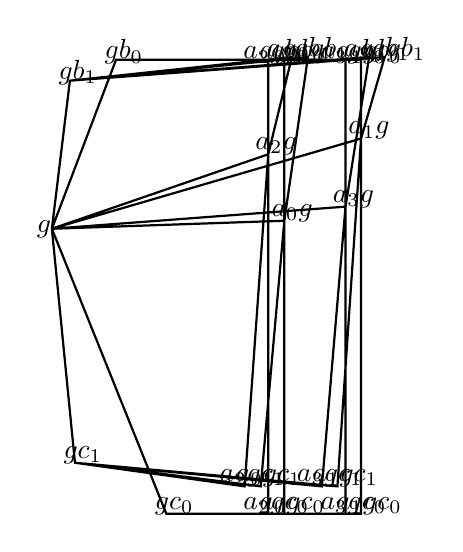
\begin{tikzpicture}
            \draw[thick](0,0)(0,0) -- (0.8145247158076414,2.145113277848677) -- (2.9522605352893745,2.145113277848677) -- (2.9522605352893745,0.1017761637518864) -- (0,0)
(0,0) -- (0.22894440168485475,1.8803677004894532) -- (3.2522605352893743,2.180367700489453) -- (2.9522605352893745,0.1017761637518864) -- (0,0)
(0,0) -- (0.8145247158076414,2.145113277848677) -- (3.926415044860695,2.145113277848677) -- (3.926415044860695,1.145711252084148) -- (0,0)
(0,0) -- (0.22894440168485475,1.8803677004894532) -- (4.226415044860695,2.180367700489453) -- (3.926415044860695,1.145711252084148) -- (0,0)
(0,0) -- (0.8145247158076414,2.145113277848677) -- (2.747941545933962,2.145113277848677) -- (2.747941545933962,0.9458945823766535) -- (0,0)
(0,0) -- (0.22894440168485475,1.8803677004894532) -- (3.047941545933962,2.180367700489453) -- (2.747941545933962,0.9458945823766535) -- (0,0)
(0,0) -- (0.8145247158076414,2.145113277848677) -- (3.7292154363868484,2.145113277848677) -- (3.7292154363868484,0.2808815448149134) -- (0,0)
(0,0) -- (0.22894440168485475,1.8803677004894532) -- (4.029215436386848,2.180367700489453) -- (3.7292154363868484,0.2808815448149134) -- (0,0)
(0,0) -- (1.4540670800540467,-3.6207613477807894) -- (2.9522605352893745,-3.6207613477807894) -- (2.9522605352893745,0.1017761637518864) -- (0,0)
(0,0) -- (0.2932294970640157,-2.9715566305180614) -- (2.6522605352893747,-3.2715566305180612) -- (2.9522605352893745,0.1017761637518864) -- (0,0)
(0,0) -- (1.4540670800540467,-3.6207613477807894) -- (3.926415044860695,-3.6207613477807894) -- (3.926415044860695,1.145711252084148) -- (0,0)
(0,0) -- (0.2932294970640157,-2.9715566305180614) -- (3.6264150448606953,-3.2715566305180612) -- (3.926415044860695,1.145711252084148) -- (0,0)
(0,0) -- (1.4540670800540467,-3.6207613477807894) -- (2.747941545933962,-3.6207613477807894) -- (2.747941545933962,0.9458945823766535) -- (0,0)
(0,0) -- (0.2932294970640157,-2.9715566305180614) -- (2.447941545933962,-3.2715566305180612) -- (2.747941545933962,0.9458945823766535) -- (0,0)
(0,0) -- (1.4540670800540467,-3.6207613477807894) -- (3.7292154363868484,-3.6207613477807894) -- (3.7292154363868484,0.2808815448149134) -- (0,0)
(0,0) -- (0.2932294970640157,-2.9715566305180614) -- (3.4292154363868486,-3.2715566305180612) -- (3.7292154363868484,0.2808815448149134) -- (0,0)
;
\node at (3.0522605352893746,2.245113277848677) {$ a_{ 0  } gb_{ 0 } $};
\node at (3.3522605352893744,2.280367700489453) {$ a_{ 0  } gb_{ 1 } $};
\node at (4.026415044860695,2.245113277848677) {$ a_{ 1  } gb_{ 0 } $};
\node at (4.326415044860695,2.280367700489453) {$ a_{ 1  } gb_{ 1 } $};
\node at (2.847941545933962,2.245113277848677) {$ a_{ 2  } gb_{ 0 } $};
\node at (3.147941545933962,2.280367700489453) {$ a_{ 2  } gb_{ 1 } $};
\node at (3.8292154363868485,2.245113277848677) {$ a_{ 3  } gb_{ 0 } $};
\node at (4.129215436386848,2.280367700489453) {$ a_{ 3  } gb_{ 1 } $};
\node at (3.0522605352893746,-3.5207613477807893) {$ a_{ 0  } gc_{ 0 } $};
\node at (2.7522605352893748,-3.171556630518061) {$ a_{ 0  } gc_{ 1 } $};
\node at (4.026415044860695,-3.5207613477807893) {$ a_{ 1  } gc_{ 0 } $};
\node at (3.7264150448606954,-3.171556630518061) {$ a_{ 1  } gc_{ 1 } $};
\node at (2.847941545933962,-3.5207613477807893) {$ a_{ 2  } gc_{ 0 } $};
\node at (2.5479415459339623,-3.171556630518061) {$ a_{ 2  } gc_{ 1 } $};
\node at (3.8292154363868485,-3.5207613477807893) {$ a_{ 3  } gc_{ 0 } $};
\node at (3.5292154363868486,-3.171556630518061) {$ a_{ 3  } gc_{ 1 } $};
\node at (-0.1,0) {$ g $};
\node at (3.0522605352893746,0.2017761637518864) {$ a_{ 0 }g $};
\node at (4.026415044860695,1.245711252084148) {$ a_{ 1 }g $};
\node at (2.847941545933962,1.0458945823766534) {$ a_{ 2 }g $};
\node at (3.8292154363868485,0.38088154481491343) {$ a_{ 3 }g $};
\node at (0.9145247158076414,2.245113277848677) {$ gb_{ 0 } $};
\node at (0.3289444016848547,1.9803677004894533) {$ gb_{ 1 } $};
\node at (1.5540670800540468,-3.5207613477807893) {$ gc_{ 0 } $};
\node at (0.39322949706401567,-2.8715566305180613) {$ gc_{ 1 } $};

            \end{tikzpicture}
            \end{center}
            \caption{Square of the complex, with edges $(g,ag), (agb, gb) \in E_A,
            (g,gb), (agb, ag) \in E_B.$ \label{fig:square}
            }
            \end{figure}
 \begin{figure}[H]
            %\label{fig:square}
            \begin{center}
            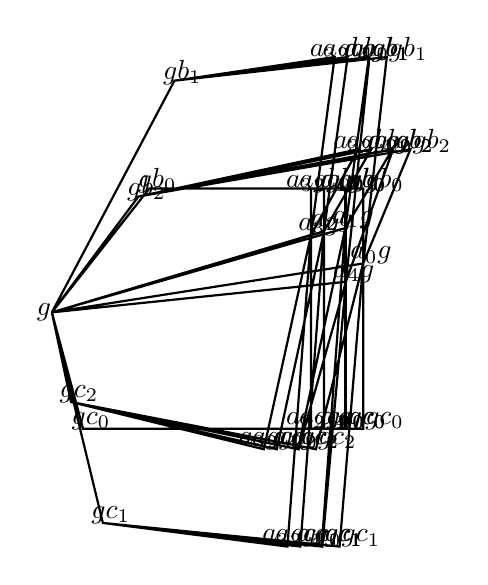
\begin{tikzpicture}
            \draw[thick](0,0)(0,0) -- (1.237470986421399,1.572917927664114) -- (3.9534255345913727,1.572917927664114) -- (3.9534255345913727,0.6207720634228632) -- (0,0)
(0,0) -- (1.5569552992433775,2.9420703102812107) -- (4.253425534591373,3.2420703102812105) -- (3.9534255345913727,0.6207720634228632) -- (0,0)
(0,0) -- (1.0996383823593776,1.471119531642647) -- (4.553425534591373,2.071119531642647) -- (3.9534255345913727,0.6207720634228632) -- (0,0)
(0,0) -- (1.237470986421399,1.572917927664114) -- (3.7262208060992896,1.572917927664114) -- (3.7262208060992896,1.0705572345590053) -- (0,0)
(0,0) -- (1.5569552992433775,2.9420703102812107) -- (4.02622080609929,3.2420703102812105) -- (3.7262208060992896,1.0705572345590053) -- (0,0)
(0,0) -- (1.0996383823593776,1.471119531642647) -- (4.32622080609929,2.071119531642647) -- (3.7262208060992896,1.0705572345590053) -- (0,0)
(0,0) -- (1.237470986421399,1.572917927664114) -- (3.4559542310086018,1.572917927664114) -- (3.4559542310086018,1.0302724053680776) -- (0,0)
(0,0) -- (1.5569552992433775,2.9420703102812107) -- (3.7559542310086016,3.2420703102812105) -- (3.4559542310086018,1.0302724053680776) -- (0,0)
(0,0) -- (1.0996383823593776,1.471119531642647) -- (4.055954231008601,2.071119531642647) -- (3.4559542310086018,1.0302724053680776) -- (0,0)
(0,0) -- (1.237470986421399,1.572917927664114) -- (3.2912940564395785,1.572917927664114) -- (3.2912940564395785,0.9833355655180995) -- (0,0)
(0,0) -- (1.5569552992433775,2.9420703102812107) -- (3.5912940564395783,3.2420703102812105) -- (3.2912940564395785,0.9833355655180995) -- (0,0)
(0,0) -- (1.0996383823593776,1.471119531642647) -- (3.8912940564395786,2.071119531642647) -- (3.2912940564395785,0.9833355655180995) -- (0,0)
(0,0) -- (1.237470986421399,1.572917927664114) -- (3.7338443377088337,1.572917927664114) -- (3.7338443377088337,0.38837968058139255) -- (0,0)
(0,0) -- (1.5569552992433775,2.9420703102812107) -- (4.0338443377088335,3.2420703102812105) -- (3.7338443377088337,0.38837968058139255) -- (0,0)
(0,0) -- (1.0996383823593776,1.471119531642647) -- (4.333844337708833,2.071119531642647) -- (3.7338443377088337,0.38837968058139255) -- (0,0)
(0,0) -- (0.39561858726331267,-1.4785448556045009) -- (3.9534255345913727,-1.4785448556045009) -- (3.9534255345913727,0.6207720634228632) -- (0,0)
(0,0) -- (0.647717053779266,-2.674472009416796) -- (3.653425534591373,-2.974472009416796) -- (3.9534255345913727,0.6207720634228632) -- (0,0)
(0,0) -- (0.24294434243257745,-1.1384007004648176) -- (3.3534255345913726,-1.7384007004648176) -- (3.9534255345913727,0.6207720634228632) -- (0,0)
(0,0) -- (0.39561858726331267,-1.4785448556045009) -- (3.7262208060992896,-1.4785448556045009) -- (3.7262208060992896,1.0705572345590053) -- (0,0)
(0,0) -- (0.647717053779266,-2.674472009416796) -- (3.42622080609929,-2.974472009416796) -- (3.7262208060992896,1.0705572345590053) -- (0,0)
(0,0) -- (0.24294434243257745,-1.1384007004648176) -- (3.1262208060992895,-1.7384007004648176) -- (3.7262208060992896,1.0705572345590053) -- (0,0)
(0,0) -- (0.39561858726331267,-1.4785448556045009) -- (3.4559542310086018,-1.4785448556045009) -- (3.4559542310086018,1.0302724053680776) -- (0,0)
(0,0) -- (0.647717053779266,-2.674472009416796) -- (3.155954231008602,-2.974472009416796) -- (3.4559542310086018,1.0302724053680776) -- (0,0)
(0,0) -- (0.24294434243257745,-1.1384007004648176) -- (2.8559542310086017,-1.7384007004648176) -- (3.4559542310086018,1.0302724053680776) -- (0,0)
(0,0) -- (0.39561858726331267,-1.4785448556045009) -- (3.2912940564395785,-1.4785448556045009) -- (3.2912940564395785,0.9833355655180995) -- (0,0)
(0,0) -- (0.647717053779266,-2.674472009416796) -- (2.9912940564395787,-2.974472009416796) -- (3.2912940564395785,0.9833355655180995) -- (0,0)
(0,0) -- (0.24294434243257745,-1.1384007004648176) -- (2.6912940564395784,-1.7384007004648176) -- (3.2912940564395785,0.9833355655180995) -- (0,0)
(0,0) -- (0.39561858726331267,-1.4785448556045009) -- (3.7338443377088337,-1.4785448556045009) -- (3.7338443377088337,0.38837968058139255) -- (0,0)
(0,0) -- (0.647717053779266,-2.674472009416796) -- (3.433844337708834,-2.974472009416796) -- (3.7338443377088337,0.38837968058139255) -- (0,0)
(0,0) -- (0.24294434243257745,-1.1384007004648176) -- (3.1338443377088336,-1.7384007004648176) -- (3.7338443377088337,0.38837968058139255) -- (0,0)
;
\node at (4.053425534591373,1.6729179276641142) {$ a_{ 0  } gb_{ 0 } $};
\node at (4.353425534591373,3.3420703102812106) {$ a_{ 0  } gb_{ 1 } $};
\node at (4.653425534591372,2.1711195316426473) {$ a_{ 0  } gb_{ 2 } $};
\node at (3.8262208060992897,1.6729179276641142) {$ a_{ 1  } gb_{ 0 } $};
\node at (4.1262208060992895,3.3420703102812106) {$ a_{ 1  } gb_{ 1 } $};
\node at (4.426220806099289,2.1711195316426473) {$ a_{ 1  } gb_{ 2 } $};
\node at (3.555954231008602,1.6729179276641142) {$ a_{ 2  } gb_{ 0 } $};
\node at (3.8559542310086017,3.3420703102812106) {$ a_{ 2  } gb_{ 1 } $};
\node at (4.155954231008601,2.1711195316426473) {$ a_{ 2  } gb_{ 2 } $};
\node at (3.3912940564395786,1.6729179276641142) {$ a_{ 3  } gb_{ 0 } $};
\node at (3.6912940564395784,3.3420703102812106) {$ a_{ 3  } gb_{ 1 } $};
\node at (3.9912940564395787,2.1711195316426473) {$ a_{ 3  } gb_{ 2 } $};
\node at (3.833844337708834,1.6729179276641142) {$ a_{ 4  } gb_{ 0 } $};
\node at (4.133844337708833,3.3420703102812106) {$ a_{ 4  } gb_{ 1 } $};
\node at (4.433844337708833,2.1711195316426473) {$ a_{ 4  } gb_{ 2 } $};
\node at (4.053425534591373,-1.3785448556045008) {$ a_{ 0  } gc_{ 0 } $};
\node at (3.753425534591373,-2.8744720094167957) {$ a_{ 0  } gc_{ 1 } $};
\node at (3.4534255345913727,-1.6384007004648176) {$ a_{ 0  } gc_{ 2 } $};
\node at (3.8262208060992897,-1.3785448556045008) {$ a_{ 1  } gc_{ 0 } $};
\node at (3.52622080609929,-2.8744720094167957) {$ a_{ 1  } gc_{ 1 } $};
\node at (3.2262208060992896,-1.6384007004648176) {$ a_{ 1  } gc_{ 2 } $};
\node at (3.555954231008602,-1.3785448556045008) {$ a_{ 2  } gc_{ 0 } $};
\node at (3.255954231008602,-2.8744720094167957) {$ a_{ 2  } gc_{ 1 } $};
\node at (2.9559542310086018,-1.6384007004648176) {$ a_{ 2  } gc_{ 2 } $};
\node at (3.3912940564395786,-1.3785448556045008) {$ a_{ 3  } gc_{ 0 } $};
\node at (3.0912940564395788,-2.8744720094167957) {$ a_{ 3  } gc_{ 1 } $};
\node at (2.7912940564395785,-1.6384007004648176) {$ a_{ 3  } gc_{ 2 } $};
\node at (3.833844337708834,-1.3785448556045008) {$ a_{ 4  } gc_{ 0 } $};
\node at (3.533844337708834,-2.8744720094167957) {$ a_{ 4  } gc_{ 1 } $};
\node at (3.2338443377088337,-1.6384007004648176) {$ a_{ 4  } gc_{ 2 } $};
\node at (-0.1,0) {$ g $};
\node at (4.053425534591373,0.7207720634228632) {$ a_{ 0 }g $};
\node at (3.8262208060992897,1.1705572345590054) {$ a_{ 1 }g $};
\node at (3.555954231008602,1.1302724053680777) {$ a_{ 2 }g $};
\node at (3.3912940564395786,1.0833355655180996) {$ a_{ 3 }g $};
\node at (3.833844337708834,0.4883796805813926) {$ a_{ 4 }g $};
\node at (1.3374709864213992,1.6729179276641142) {$ gb_{ 0 } $};
\node at (1.6569552992433776,3.0420703102812108) {$ gb_{ 1 } $};
\node at (1.1996383823593777,1.5711195316426472) {$ gb_{ 2 } $};
\node at (0.49561858726331265,-1.3785448556045008) {$ gc_{ 0 } $};
\node at (0.747717053779266,-2.574472009416796) {$ gc_{ 1 } $};
\node at (0.34294434243257743,-1.0384007004648175) {$ gc_{ 2 } $};

            \end{tikzpicture}
            \end{center}
            \caption{Square of the complex, with edges $(g,ag), (agb, gb) \in E_A,
            (g,gb), (agb, ag) \in E_B.$ \label{fig:square}
            }
            \end{figure}
 \begin{figure}[H]
            %\label{fig:square}
            \begin{center}
            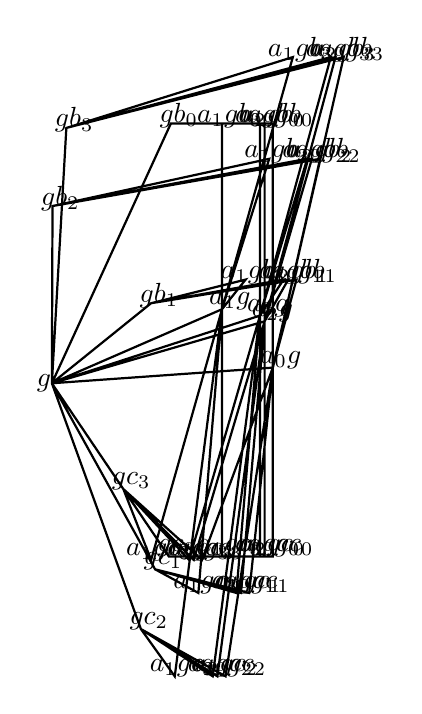
\begin{tikzpicture}
            \draw[thick](0,0)(0,0) -- (1.5115846149638696,3.2995297303565576) -- (2.806113910874833,3.2995297303565576) -- (2.806113910874833,0.19845650743649612) -- (0,0)
(0,0) -- (1.260208295338278,1.0165349630088047) -- (3.106113910874833,1.3165349630088048) -- (2.806113910874833,0.19845650743649612) -- (0,0)
(0,0) -- (0.008081036722000112,2.250547556187305) -- (3.4061139108748333,2.8505475561873053) -- (2.806113910874833,0.19845650743649612) -- (0,0)
(0,0) -- (0.1838610376544374,3.2425295817098636) -- (3.706113910874833,4.142529581709864) -- (2.806113910874833,0.19845650743649612) -- (0,0)
(0,0) -- (1.5115846149638696,3.2995297303565576) -- (2.1606075025312683,3.2995297303565576) -- (2.1606075025312683,0.9400140593564503) -- (0,0)
(0,0) -- (1.260208295338278,1.0165349630088047) -- (2.460607502531268,1.3165349630088048) -- (2.1606075025312683,0.9400140593564503) -- (0,0)
(0,0) -- (0.008081036722000112,2.250547556187305) -- (2.7606075025312684,2.8505475561873053) -- (2.1606075025312683,0.9400140593564503) -- (0,0)
(0,0) -- (0.1838610376544374,3.2425295817098636) -- (3.0606075025312682,4.142529581709864) -- (2.1606075025312683,0.9400140593564503) -- (0,0)
(0,0) -- (1.5115846149638696,3.2995297303565576) -- (2.701858384810507,3.2995297303565576) -- (2.701858384810507,0.7868606013599231) -- (0,0)
(0,0) -- (1.260208295338278,1.0165349630088047) -- (3.001858384810507,1.3165349630088048) -- (2.701858384810507,0.7868606013599231) -- (0,0)
(0,0) -- (0.008081036722000112,2.250547556187305) -- (3.301858384810507,2.8505475561873053) -- (2.701858384810507,0.7868606013599231) -- (0,0)
(0,0) -- (0.1838610376544374,3.2425295817098636) -- (3.601858384810507,4.142529581709864) -- (2.701858384810507,0.7868606013599231) -- (0,0)
(0,0) -- (1.5115846149638696,3.2995297303565576) -- (2.6428207258798704,3.2995297303565576) -- (2.6428207258798704,0.8588754055618403) -- (0,0)
(0,0) -- (1.260208295338278,1.0165349630088047) -- (2.94282072587987,1.3165349630088048) -- (2.6428207258798704,0.8588754055618403) -- (0,0)
(0,0) -- (0.008081036722000112,2.250547556187305) -- (3.2428207258798705,2.8505475561873053) -- (2.6428207258798704,0.8588754055618403) -- (0,0)
(0,0) -- (0.1838610376544374,3.2425295817098636) -- (3.5428207258798703,4.142529581709864) -- (2.6428207258798704,0.8588754055618403) -- (0,0)
(0,0) -- (1.4853596074397635,-2.199384078450705) -- (2.806113910874833,-2.199384078450705) -- (2.806113910874833,0.19845650743649612) -- (0,0)
(0,0) -- (1.3108444254389848,-2.362769103613562) -- (2.5061139108748334,-2.6627691036135617) -- (2.806113910874833,0.19845650743649612) -- (0,0)
(0,0) -- (1.1310744230858478,-3.1216855064753712) -- (2.206113910874833,-3.7216855064753713) -- (2.806113910874833,0.19845650743649612) -- (0,0)
(0,0) -- (0.9074589828184634,-1.3430652315526261) -- (1.9061139108748333,-2.243065231552626) -- (2.806113910874833,0.19845650743649612) -- (0,0)
(0,0) -- (1.4853596074397635,-2.199384078450705) -- (2.1606075025312683,-2.199384078450705) -- (2.1606075025312683,0.9400140593564503) -- (0,0)
(0,0) -- (1.3108444254389848,-2.362769103613562) -- (1.8606075025312683,-2.6627691036135617) -- (2.1606075025312683,0.9400140593564503) -- (0,0)
(0,0) -- (1.1310744230858478,-3.1216855064753712) -- (1.5606075025312682,-3.7216855064753713) -- (2.1606075025312683,0.9400140593564503) -- (0,0)
(0,0) -- (0.9074589828184634,-1.3430652315526261) -- (1.2606075025312684,-2.243065231552626) -- (2.1606075025312683,0.9400140593564503) -- (0,0)
(0,0) -- (1.4853596074397635,-2.199384078450705) -- (2.701858384810507,-2.199384078450705) -- (2.701858384810507,0.7868606013599231) -- (0,0)
(0,0) -- (1.3108444254389848,-2.362769103613562) -- (2.4018583848105073,-2.6627691036135617) -- (2.701858384810507,0.7868606013599231) -- (0,0)
(0,0) -- (1.1310744230858478,-3.1216855064753712) -- (2.101858384810507,-3.7216855064753713) -- (2.701858384810507,0.7868606013599231) -- (0,0)
(0,0) -- (0.9074589828184634,-1.3430652315526261) -- (1.8018583848105072,-2.243065231552626) -- (2.701858384810507,0.7868606013599231) -- (0,0)
(0,0) -- (1.4853596074397635,-2.199384078450705) -- (2.6428207258798704,-2.199384078450705) -- (2.6428207258798704,0.8588754055618403) -- (0,0)
(0,0) -- (1.3108444254389848,-2.362769103613562) -- (2.3428207258798706,-2.6627691036135617) -- (2.6428207258798704,0.8588754055618403) -- (0,0)
(0,0) -- (1.1310744230858478,-3.1216855064753712) -- (2.0428207258798703,-3.7216855064753713) -- (2.6428207258798704,0.8588754055618403) -- (0,0)
(0,0) -- (0.9074589828184634,-1.3430652315526261) -- (1.7428207258798705,-2.243065231552626) -- (2.6428207258798704,0.8588754055618403) -- (0,0)
;
\node at (2.9061139108748333,3.3995297303565577) {$ a_{ 0  } gb_{ 0 } $};
\node at (3.206113910874833,1.4165349630088049) {$ a_{ 0  } gb_{ 1 } $};
\node at (3.5061139108748334,2.9505475561873054) {$ a_{ 0  } gb_{ 2 } $};
\node at (3.806113910874833,4.242529581709864) {$ a_{ 0  } gb_{ 3 } $};
\node at (2.2606075025312684,3.3995297303565577) {$ a_{ 1  } gb_{ 0 } $};
\node at (2.5606075025312682,1.4165349630088049) {$ a_{ 1  } gb_{ 1 } $};
\node at (2.8606075025312685,2.9505475561873054) {$ a_{ 1  } gb_{ 2 } $};
\node at (3.1606075025312683,4.242529581709864) {$ a_{ 1  } gb_{ 3 } $};
\node at (2.801858384810507,3.3995297303565577) {$ a_{ 2  } gb_{ 0 } $};
\node at (3.101858384810507,1.4165349630088049) {$ a_{ 2  } gb_{ 1 } $};
\node at (3.4018583848105073,2.9505475561873054) {$ a_{ 2  } gb_{ 2 } $};
\node at (3.701858384810507,4.242529581709864) {$ a_{ 2  } gb_{ 3 } $};
\node at (2.7428207258798705,3.3995297303565577) {$ a_{ 3  } gb_{ 0 } $};
\node at (3.0428207258798703,1.4165349630088049) {$ a_{ 3  } gb_{ 1 } $};
\node at (3.3428207258798706,2.9505475561873054) {$ a_{ 3  } gb_{ 2 } $};
\node at (3.6428207258798704,4.242529581709864) {$ a_{ 3  } gb_{ 3 } $};
\node at (2.9061139108748333,-2.0993840784507047) {$ a_{ 0  } gc_{ 0 } $};
\node at (2.6061139108748335,-2.5627691036135616) {$ a_{ 0  } gc_{ 1 } $};
\node at (2.306113910874833,-3.6216855064753712) {$ a_{ 0  } gc_{ 2 } $};
\node at (2.0061139108748334,-2.143065231552626) {$ a_{ 0  } gc_{ 3 } $};
\node at (2.2606075025312684,-2.0993840784507047) {$ a_{ 1  } gc_{ 0 } $};
\node at (1.9606075025312684,-2.5627691036135616) {$ a_{ 1  } gc_{ 1 } $};
\node at (1.6606075025312683,-3.6216855064753712) {$ a_{ 1  } gc_{ 2 } $};
\node at (1.3606075025312685,-2.143065231552626) {$ a_{ 1  } gc_{ 3 } $};
\node at (2.801858384810507,-2.0993840784507047) {$ a_{ 2  } gc_{ 0 } $};
\node at (2.5018583848105074,-2.5627691036135616) {$ a_{ 2  } gc_{ 1 } $};
\node at (2.201858384810507,-3.6216855064753712) {$ a_{ 2  } gc_{ 2 } $};
\node at (1.9018583848105073,-2.143065231552626) {$ a_{ 2  } gc_{ 3 } $};
\node at (2.7428207258798705,-2.0993840784507047) {$ a_{ 3  } gc_{ 0 } $};
\node at (2.4428207258798706,-2.5627691036135616) {$ a_{ 3  } gc_{ 1 } $};
\node at (2.1428207258798704,-3.6216855064753712) {$ a_{ 3  } gc_{ 2 } $};
\node at (1.8428207258798706,-2.143065231552626) {$ a_{ 3  } gc_{ 3 } $};
\node at (-0.1,0) {$ g $};
\node at (2.9061139108748333,0.2984565074364961) {$ a_{ 0 }g $};
\node at (2.2606075025312684,1.0400140593564504) {$ a_{ 1 }g $};
\node at (2.801858384810507,0.8868606013599231) {$ a_{ 2 }g $};
\node at (2.7428207258798705,0.9588754055618403) {$ a_{ 3 }g $};
\node at (1.6115846149638697,3.3995297303565577) {$ gb_{ 0 } $};
\node at (1.3602082953382781,1.1165349630088048) {$ gb_{ 1 } $};
\node at (0.10808103672200012,2.3505475561873053) {$ gb_{ 2 } $};
\node at (0.2838610376544374,3.3425295817098637) {$ gb_{ 3 } $};
\node at (1.5853596074397636,-2.0993840784507047) {$ gc_{ 0 } $};
\node at (1.410844425438985,-2.2627691036135618) {$ gc_{ 1 } $};
\node at (1.231074423085848,-3.021685506475371) {$ gc_{ 2 } $};
\node at (1.0074589828184635,-1.243065231552626) {$ gc_{ 3 } $};

            \end{tikzpicture}
            \end{center}
            \caption{Square of the complex, with edges $(g,ag), (agb, gb) \in E_A,
            (g,gb), (agb, ag) \in E_B.$ \label{fig:square}
            }
            \end{figure}
 
\end{multicols*}
  % \printbibliography 
\end{document}

 